\documentclass[a4paper, 12pt]{article}

\usepackage{geometry}
\usepackage{graphicx}
\usepackage{hyperref}
\usepackage{listings}
\usepackage{mathtools}
\usepackage{titling}

\newcommand{\subtitle}[1]{% 
	\posttitle{%
		\par \end{center}
		\begin{center}\small#1\end{center}
		\vskip7em}%
}


\begin{document}
\pagenumbering{gobble}
% Page 1 - Titles

\title{\Large Digital Signal Processing Project on}
\subtitle{\Huge Huffman Encoding \& Decoding using MATLAB}
\author{\LARGE By:  Ravi Teja Gannavarapu}
\date{\Large Student ID: B216023}
\maketitle

\begin{center}
\vskip2em
\Large Branch: Electronics \& Telecommunication Engineering
\newline
Class: 2016 - 2020
\end{center}

\begin{center}
\vskip4em
\large International Institute of Information Technology, Bhubaneswar
\newline
Gothapatna, PO: Mailpada, Bhubaneswar.
\end{center}

\pagebreak
% Page 2 - Abstract

\newgeometry{left=1cm, right=1cm, top=2cm, bottom=2cm}
\pagenumbering{arabic}
\begin{center}
\LARGE Huffman Encoding \& Decoding using MATLAB\\\rule{19cm}{0.01cm}
\end{center}
\begin{center}
\Large Abstract\\\rule{19cm}{0.01cm}\\\vskip2em
\end{center}

\Large Data, when being transmitted over large distances and via different channels, requires to be sent securely. Encoding the
information before transmission is necessary to ensure data security and efficient delivery of the information. \textbf{Huffman algorithm} is a popular encoding method used in communication systems. Huffman encoding and decoding algorithm is used in compressing data with variable-length codes. The shortest codes are assigned to the most frequent characters and the longest codes are assigned to infrequent characters. Huffman coding is an entropy encoding algorithm used for \textbf{lossless} data compression. \textbf{Entropy} is a measure of the unpredictability of an information stream. Maximum entropy occurs when a stream of data has totally unpredictable bits. A perfectly consistent stream of bits (all zeroes or all ones) is totally predictable, and has no entropy.

\pagebreak
% Page 3 - Introduction

\begin{center}
\LARGE Huffman Encoding \& Decoding using MATLAB\\\rule{19cm}{0.01cm}
\end{center}
\begin{center}
\Large Introduction\\\rule{19cm}{0.01cm}\\\vskip2em
\end{center}

\Large Encoding the information before transmission is necessary to ensure data security and efficient delivery of the information. The MATLAB program presented further encodes and decodes the information and also outputs the values of \textbf{entropy, efficiency} and \textbf{frequency probabilities} of characters present in the data stream.
\newline
\newline

Huffman algorithm is a popular encoding method used in communication systems. It is widely used in all the mainstream compression formats that you might encounter - from GZIP, PKZIP and BZIP2, to image formats such as JPEG and PNG. Some programs use just the Huffman coding method, while others use it as one step in a multistep compression process.
\newline
\newline

Huffman encoding \& decoding algorithm is used in compressing data with variable-length codes. The shortest codes are assigned to the most frequent characters and the longest codes are assigned to infrequent characters.
\newline
\newline

Huffman coding is an entropy encoding algorithm used for lossless data compression. \textbf{Entropy} is a measure of the unpredictability of an information stream. Maximum entropy occurs when a stream of data has totally unpredictable bits. A perfectly consistent stream of bits (all zeroes or all ones) is totally predictable (has no entropy).

\pagebreak
% Page 4 - Huffman Tree

\begin{center}
\LARGE Huffman Encoding \& Decoding using MATLAB\\\rule{19cm}{0.01cm}
\end{center}
\begin{center}
\Large Huffman Tree\\\rule{19cm}{0.01cm}\\\vskip2em
\end{center}

\Large The Huffman coding method is somewhat similar to the Shannon–Fano method. The main difference between the two methods is that Shannon–Fano constructs its codes from top to bottom (and the bits of each codeword are constructed from left to right), while Huffman constructs a code tree from the bottom up and the bits of each codeword are constructed from right to left.
\newline
\newline

The simplest tree construction algorithm uses a priority queue or table where the node with the lowest probability or frequency is given the highest priority. First, create a leaf node for each symbol or character and add it to the priority table. If there is more than one node in the table, remove two nodes of the highest priority (lowest frequency) from the table. Create a new node with these two nodes as sub-nodes and with probability equal to the sum of the two nodes’ probabilities. Continue in this way until you reach the last single node. The last node is the root, so the tree is now complete.
\newline
\newline

\begin{center}
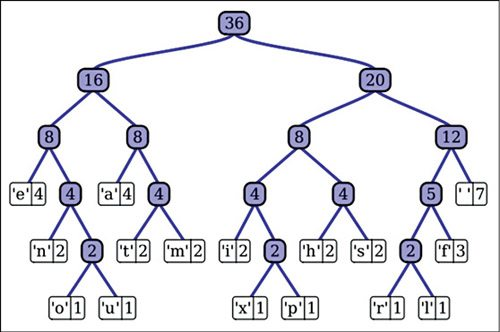
\includegraphics[width=250px]{huffmantree.jpg}
\end{center}
\begin{center}
\large Figure 1: Huffman Tree.
\end{center}

\pagebreak
% Page 5 - Steps to encode

\begin{center}
\LARGE Huffman Encoding \& Decoding using MATLAB\\\rule{19cm}{0.01cm}
\end{center}
\begin{center}
\Large Steps to encode\\\rule{19cm}{0.01cm}\\\vskip2em
\end{center}

\begin{enumerate}
\item Compute the probability of each character in a set of data.
\item Sort the set of data in ascending order.
\item Create a new node where the left sub-node is the lowest frequency in the sorted list and the right sub-node is the second lowest in the sorted list.
\item Remove these two elements from the sorted list as they are now part of one node and add the probabilities. The result is the probability for the new node.
\item Perform insertion sort on the list.
\item Repeat steps 3, 4 and 5 until you have only one node left.
\end{enumerate}

Now that there is one node remaining, simply draw the tree. With the above tree, place a ‘0’ on each path going to the left and a ‘1’ on each path going to the right. Now assign the binary code to each of the symbols or characters by counting 0’s and 1’s starting from the root
\newline
\newline

From the above, it is now clear that the encoding method should give rise to a uniquely decodable code so that the original message can be detected uniquely and perfectly without errors. The message generated with the highest probability will be generated more number of times than other messages. In such a case, if you use a variable-length code instead of a fixed-length code, you will be improving the efficiency by assigning fewer bits to the higher-probability messages than the lower-probability messages.

\pagebreak
% Page 6 - How the MATLAB code works

\begin{center}
\LARGE Huffman Encoding \& Decoding using MATLAB\\\rule{19cm}{0.01cm}
\end{center}
\begin{center}
\Large How the MATLAB code works?\\\rule{19cm}{0.01cm}\\\vskip2em
\end{center}

\begin{enumerate}
\item List the source probabilities in decreasing order.
\item Combine the probabilities of the two symbols having the lowest probabilities, and record the resultant probabilities; this step is called reduction. This procedure is repeated until there are two-order probabilities remaining.
\item Start encoding with the last reduction, which consists of exactly two-order probabilities. Assign ‘0’ as the first digit in the code words for all the source symbols associated with the first probability; assign ‘1’ to the second probability.
\item Now go back and assign ‘0’ and ‘1’ to the second digit for the two probabilities that were combined in the previous reduction step, retaining all assignments made in Step 3.
\item Keep regressing in this way until the first column is reached.
\item Calculate the entropy. The entropy of the code is the average number of bits needed to decode a given pattern.
\item Calculate efficiency. For evaluating the source code generated, you need to calculate its efficiency.
\end{enumerate}

Efficiency = Entropy (H(X)) / Average codeword length (N)

\begin{align*}
N &= \sum_{i=0}^{n} P_{i} * N_{i}
\end{align*}

where N\textsubscript{i} is the length of \textit{ith} codeword and P\textsubscript{i} is the probability of occurence.

\pagebreak
% Page 7 - MATLAB functions

\begin{center}
\LARGE Huffman Encoding \& Decoding using MATLAB\\\rule{19cm}{0.01cm}
\end{center}
\begin{center}
\Large MATLAB functions explained\\\rule{19cm}{0.01cm}\\\vskip2em
\end{center}

\textbf {huffmanenco}: This function is used in Huffman encoding. The syntax is:
\begin{center}
\texttt{comp = huffmanenco(sig, dict)}
\end{center}

This line encodes the signal 'sig' described by the 'dict' dictionary. The argument 'sig' can have the form of a numeric vector, numeric cell array or alphanumeric cell array. If 'sig' is a cell array, it must be either a row or a column. The 'dict' is an Nx2 cell array, where 'N' is the number of distinct possible symbols to be encoded. The first column of 'dict' represents the distinct symbols and the second column represents the corresponding codewords. Each codeword is represented as a numeric row vector, and no codeword in 'dict' can be the prefix of any other codeword in 'dict'. You can generate 'dict' using the huffmandict function.
\newline
\newline

\textbf {huffmandeco}: This function is used in Huffman decoding. The syntax is:
\begin{center}
\texttt{dsig = huffmandeco(comp, dict)}
\end{center}

This line decodes the numeric Huffman code vector comp using the code dictionary 'dict'. The argument 'dict' is an Nx2 cell array, where 'N' is the number of distinct possible symbols in the original signal that was encoded as 'comp'. The first column of 'dict' represents the distinct symbols and the second column represents the corresponding codewords. Each codeword is represented as a numeric row vector, and no codeword in 'dict' is allowed to be the prefix of any other codeword in 'dict'. You can generate 'dict' using the Huffmandict function and 'comp' using the huffmanenco function. If all signal values in 'dict' are numeric, 'dsig' is a vector; if any signal value in 'dict' is alphabetical, 'dsig' is a one-dimensional cell array.

\pagebreak
% Page 8 - MATLAB Code

\begin{center}
\LARGE Huffman Encoding \& Decoding using MATLAB\\\rule{19cm}{0.01cm}
\end{center}
\begin{center}
\Large MATLAB Code\\\rule{19cm}{0.01cm}\\\vskip1em
\end{center}

\small \begin{lstlisting}[language=Matlab]
clc;
clearvars;
close all;

p = input('Enter the probabilities: ');
n = length(p);
symbols = [1:n];
[dict, avglen] = huffmandict(symbols, p);
temp = dict;
t = dict(:,2);

for i = 1:length(temp)
    temp{i,2} = num2str(temp{i,2});
end

disp('The Huffman code dict is: ');
disp(temp)

% Encoder
fprintf('Enter a symbol between 1 to %d as array:', n);
sym = input(' ');
encod = huffmanenco(sym, dict);
disp('The encoded output: ');
disp(encod);

% Decoder
bits = input('Enter the encoded bit stream as array: ');
decod = huffmandeco(bits, dict);
fprintf('The decoded symbols are: %d\n', decod);

H = 0;
for k = 1:n
    H = H + (p(k)*log2(1/p(k)));
end
fprintf('Entropy is %f bits\n', H);
N = H / avglen;
fprintf('Efficiency is: %f\n', N);
for r = 1:n
   l(r) = length(t{r});
end
m = max(l);
s = min(l);
v = m-s; % Variance
fprintf('The variance is: %d\n', v);
\end{lstlisting}

\pagebreak
% Page 9 -  Output, conclusion & future scope

\begin{center}
\LARGE Huffman Encoding \& Decoding using MATLAB\\\rule{19cm}{0.01cm}
\end{center}
\begin{center}
\Large Output, Conclusion \& Future Scope\\\rule{19cm}{0.01cm}\\\vskip2em
\end{center}

\begin{center}
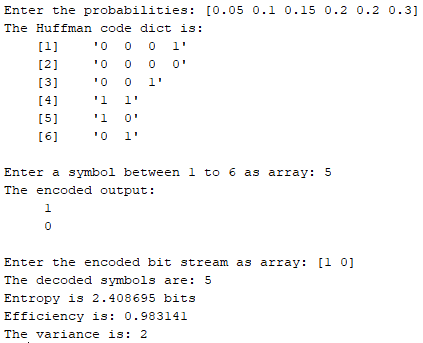
\includegraphics[width=330px]{output.png}
\end{center}
\begin{center}
\large Figure 2: MATLAB Output.
\end{center}
\vskip2em

\Large \textbf{Conclusion}: Huffman encoding is a very effective compression algorithm for lossless compression. This can be used to send data over various channels without the risk of data loss.
\newline
\newline

\Large \textbf{Future scope}: Huffman encoding can be used further as one of the steps in a multistep compression process, thus helping reduce the payload size when transmitting data over long distances. This not only decreases the transmission delays but also increases the overall speed of the network because the overall data size is way less because the data is now highly compressed.

\pagebreak
% Page 10 -  References

\begin{center}
\LARGE Huffman Encoding \& Decoding using MATLAB\\\rule{19cm}{0.01cm}
\end{center}
\begin{center}
\Large References\\\rule{19cm}{0.01cm}\\\vskip2em
\end{center}

\begin{enumerate}
\item ElectronicsForU - \href{https://electronicsforu.com/electronics-projects/software-projects-ideas/huffman-coding-decoding-matlab/}{Huffman Encoding \& Decoding in MATLAB}
\item Wikipedia - \href{https://en.wikipedia.org/wiki/Huffman_coding}{Huffman Coding}
\item MathWorks - \href{https://in.mathworks.com/help/comm/ref/huffmanenco.html}{Huffman Encoding}
\item MathWorks - \href{https://in.mathworks.com/help/comm/ref/huffmandeco.html}{Huffman Decoding}
\end{enumerate}

\end{document}